\documentclass[11pt]{article}

\usepackage[utf8]{inputenc}
\usepackage[T1]{fontenc}
\usepackage{lmodern}
\usepackage[margin=1in]{geometry}
\usepackage{amsmath,amssymb,amsthm,mathtools}
\usepackage{booktabs,tabularx,array}
\usepackage{xcolor}
\usepackage{listings}
\usepackage{tikz}
\usetikzlibrary{arrows.meta,positioning,fit}
\usepackage{microtype}
\usepackage[hidelinks]{hyperref}
\usepackage[nameinlink,capitalise]{cleveref}
\usepackage{enumitem}
\usepackage[numbers,sort&compress]{natbib}

% ---------------------------------------------------------------------------
% Lean listings (pdflatex-compatible: Unicode via literate replacements)
\definecolor{leankw}{RGB}{0,0,160}
\definecolor{leancomment}{RGB}{90,90,90}
\lstdefinelanguage{lean}{
  keywords={theorem,lemma,def,noncomputable,structure,where,fun,by,let,have,show,
    if,then,else,namespace,end,open,import,variable,abbrev,Prop,Type,section},
  sensitive=true,
  morecomment=[l]{--},
  morecomment=[s]{/-}{-/},
  morestring=[b]",
}
\lstset{
  language=lean,
  basicstyle=\ttfamily\small,
  keywordstyle=\color{leankw}\bfseries,
  commentstyle=\color{leancomment}\itshape,
  columns=fullflexible,
  keepspaces=true,
  breaklines=true,
  breakatwhitespace=false,
  postbreak=\mbox{\textcolor{leancomment}{$\hookrightarrow$}\space},
  frame=single,
  framesep=4pt,
  rulecolor=\color{black!30},
  xleftmargin=6pt,
  xrightmargin=6pt,
  aboveskip=8pt,
  belowskip=8pt,
  extendedchars=true,
  inputencoding=utf8,
  literate=
    {ℝ}{{$\mathbb{R}$}}1 {ℕ}{{$\mathbb{N}$}}1
    {→}{{$\to$}}1 {←}{{$\leftarrow$}}1 {↦}{{$\mapsto$}}1
    {∀}{{$\forall$}}1 {∃}{{$\exists$}}1 {∑}{{$\Sigma$}}1
    {≠}{{$\neq$}}1 {≤}{{$\le$}}1 {≥}{{$\ge$}}1
    {⟨}{{$\langle$}}1 {⟩}{{$\rangle$}}1
    {∧}{{$\wedge$}}1 {∨}{{$\vee$}}1 {¬}{{$\neg$}}1
    {·}{{$\cdot$}}1 {•}{{$\bullet$}}1 {∘}{{$\circ$}}1 {×}{{$\times$}}1
    {√}{{$\surd$}}1 {∂}{{$\partial$}}1 {♯}{{$\sharp$}}1 {⋆}{{$\star$}}1
    {⁻¹}{{$^{-1}$}}2 {²}{{$^2$}}1 {³}{{$^3$}}1 {⁴}{{$^4$}}1
    {₀}{{$_0$}}1 {₁}{{$_1$}}1 {₂}{{$_2$}}1 {₃}{{$_3$}}1 {₊}{{$_+$}}1
    {ᶠ}{{$^{f}$}}1
    {α}{{$\alpha$}}1 {β}{{$\beta$}}1 {γ}{{$\gamma$}}1 {δ}{{$\delta$}}1
    {ε}{{$\varepsilon$}}1 {η}{{$\eta$}}1 {λ}{{$\lambda$}}1 {μ}{{$\mu$}}1
    {ν}{{$\nu$}}1 {ρ}{{$\rho$}}1 {σ}{{$\sigma$}}1 {φ}{{$\varphi$}}1
    {ψ}{{$\psi$}}1 {Γ}{{$\Gamma$}}1 {Φ}{{$\Phi$}}1
    {½}{{$\frac12$}}1 {¼}{{$\frac14$}}1
    {–}{{--}}1 {—}{{---}}1 {…}{{\ldots}}1
}

% ---------------------------------------------------------------------------
\newtheorem{theorem}{Theorem}[section]
\newtheorem{lemma}[theorem]{Lemma}
\newtheorem{proposition}[theorem]{Proposition}
\newtheorem{corollary}[theorem]{Corollary}
\theoremstyle{definition}
\newtheorem{definition}[theorem]{Definition}
\theoremstyle{remark}
\newtheorem{remark}[theorem]{Remark}

\newcommand{\R}{\mathbb{R}}
\newcommand{\Q}{\mathbb{Q}}
\newcommand{\lean}[1]{\lstinline[basicstyle=\ttfamily\normalsize,columns=fullflexible,breaklines=false]{#1}}
\newcommand{\ksharp}{k^{\sharp}}
\newcommand{\LM}{\operatorname{LM}}
\newcommand{\NF}{\operatorname{NF}}

% Statistics (filled from the measured data; see the accompanying README)
% provisional values -- to be replaced by measured data
\newcommand{\EinsteinKB}{980}
\newcommand{\NoveltySentence}{}
\newcommand{\ConventionsSentence}{}
\newcommand{\NumLCEinstein}{166}
\newcommand{\ClosedFormStats}{}
\newcommand{\NumLinesFieldClosed}{88}
\newcommand{\NumLinesMaxwell}{460}
\newcommand{\NumLinesFlatMaxwell}{720}
\newcommand{\NumLinesFinal}{251}
\newcommand{\StatsTable}{}
\newcommand{\AxiomsOutput}{\begin{lstlisting}
'solution' depends on axioms: [propext, Classical.choice, Quot.sound]
\end{lstlisting}}
\newcommand{\LocalCheckSentence}{}
\newcommand{\RelatedFormalPhysics}{TBD.}
\newcommand{\RepoNote}{}


\title{A Machine-Checked Proof that the Kerr--Newman Spacetime\\ Solves the Einstein--Maxwell Equations}
\author{Samen Hossain}
\date{October 2026}

\begin{document}
\maketitle

\begin{abstract}
We present a complete formal proof, in the Lean~4 proof assistant with the Mathlib library, that the Kerr--Newman metric and its electromagnetic field satisfy the Einstein--Maxwell equations.
The statement is phrased in Kerr--Schild Cartesian coordinates on $\R^4$.
It holds for all real mass, spin and charge parameters $(m,a,e)$, at every point where the Kerr--Schild radial function is positive.
It has three parts: the Einstein equation $G_{\mu\nu}=8\pi T_{\mu\nu}$ with the electromagnetic stress--energy tensor, the source-free Maxwell equation $\partial_\mu(\sqrt{|\det g|}\,F^{\mu\nu})=0$, and closedness of $F$.
Christoffel symbols, curvature and all derivatives are defined from first principles through Fr\'echet derivatives.
The proof uses no axioms beyond the three standard ones of Lean.

The obstacle is the size of the curvature computation, which computer algebra performs routinely but which is far beyond what can be written by hand in a proof assistant.
We overcome it by expressing every quantity as a polynomial in five \emph{atoms}: the radial function~$r$, the spatial components of the Kerr--Schild null covector, and $W=1/(r^2+a^2\cos^2\theta)$.
The atoms are closed under differentiation and satisfy two polynomial relations.
This turns each step of the curvature computation into an identity in a quotient ring.
Each identity is certified by cofactors from Gr\"obner-basis division, computed offline with SymPy and checked in Lean by \lean{linear_combination}, so the computer algebra system is never trusted.
The Maxwell equations are proved conceptually: the Kerr--Schild structure reduces the curved equation to the flat one, which follows from the harmonicity of Appell's complex-shifted Coulomb potential.
We describe the method, the engineering needed to fit about one megabyte of mostly generated Lean into a 300-second per-file checking budget, and the trusted base of the result.
The formalization was produced by an AI coding agent on the Prove2Me platform under the author's direction, and we document that process.
\end{abstract}

\tableofcontents

% ===========================================================================
\section{Introduction}\label{sec:intro}

In 1963 Kerr found the metric of a rotating black hole~\cite{kerr1963}.
Two years later Newman and collaborators found its electrically charged generalization~\cite{newman1965}.
The resulting Kerr--Newman family is labelled by a mass~$m$, a spin parameter~$a$ (angular momentum per unit mass) and a charge~$e$.
It plays a distinguished role because of the black-hole uniqueness theorems~\cite{israel1967,israel1968,carter1971,hawking1972,robinson1975,mazur1982,bunting1983}.
Under suitable regularity and global assumptions, these theorems show that Kerr--Newman metrics exhaust the stationary, asymptotically flat black-hole solutions of the Einstein--Maxwell equations.
This is the ``no-hair'' property; see the review~\cite{chrusciel2012} for the precise hypotheses and for the questions that remain open.

The most basic fact about an exact solution is that it actually solves the field equations.
For Kerr--Newman this is a substantial calculation.
One computes forty independent Christoffel symbols, their derivatives and the Ricci tensor, and then compares the result with the electromagnetic stress--energy tensor.
Every intermediate quantity is a sizeable rational function of the coordinates.
In practice the check is left to computer algebra systems~\cite{maccallum2018}.
These are reliable, but they do not produce a proof that can be checked independently.
Interactive theorem provers such as Lean~\cite{demoura2021} reduce trust to a small proof-checking kernel.
So far they have been used little for heavy computations in general relativity (\cref{sec:related}).

\paragraph{Result.}
We report a complete formal proof of the following statement.
The precise Lean statement and all the definitions it uses are reproduced in \cref{sec:statement,app:defs}.

\begin{theorem}[informal]\label{thm:main}
Let $m,a,e\in\R$.
Let $g$ be the Kerr--Newman metric in Kerr--Schild coordinates, and let $F=dA$ be the Kerr--Newman electromagnetic field.
Then at every point $p\in\R^4$ where the Kerr--Schild radius satisfies $r(p)>0$:
\begin{enumerate}[label=(\roman*)]
  \item $G_{\mu\nu} = 2\big(F_{\mu\alpha}F_{\nu}{}^{\alpha} - \tfrac14\, g_{\mu\nu}F_{\alpha\beta}F^{\alpha\beta}\big)$, that is, $G_{\mu\nu}=8\pi T_{\mu\nu}$ in Gaussian geometrized units;
  \item $\partial_\mu\big(\sqrt{|\det g|}\,F^{\mu\nu}\big)=0$ for every $\nu$;
  \item $\partial_\lambda F_{\mu\nu}+\partial_\mu F_{\nu\lambda}+\partial_\nu F_{\lambda\mu}=0$ for all $\lambda,\mu,\nu$.
\end{enumerate}
\end{theorem}

The theorem places no restriction on the parameters.
It therefore covers black holes ($a^2+e^2\le m^2$) as well as over-extremal and negative-mass members of the family.
It holds everywhere in the Kerr--Schild chart except on the disc spanned by the ring singularity, including inside the horizons.
All derivatives are genuine Fr\'echet derivatives, the inverse metric is the matrix inverse, and curvature follows the textbook coordinate formulas.
The kernel accepts the proof with only the axioms \lean{propext}, \lean{Classical.choice} and \lean{Quot.sound}.

\paragraph{Contributions.}
\begin{itemize}
  \item A complete, kernel-checked proof of \cref{thm:main} in Lean~4 and Mathlib~\cite{mathlib2020} (\cref{sec:einstein,sec:maxwell}).
  To our knowledge, no earlier machine-checked proof shows that Kerr--Newman, Kerr or even Schwarzschild satisfies the Einstein equations with the curvature computed from the metric by the prover's own calculus (\cref{sec:related}).
  \item A method for curvature computations in a proof assistant that keeps the computer algebra system outside the trusted base (\cref{sec:atoms,sec:certificates,sec:hascp}).
  Every quantity is written in a small set of algebraically constrained \emph{atoms} that is closed under differentiation.
  Each identity is then a polynomial ideal-membership problem, certified by Gr\"obner-basis cofactors and replayed by Lean's \lean{linear_combination} tactic.
  \item A short conceptual proof of the Maxwell equations (\cref{sec:maxwell}).
  It rests on two classical facts: the reduction of the curved equation to the flat one for Kerr--Schild fields aligned with~$k$, and Appell's interpretation of the Kerr--Newman potential as a Coulomb potential centred at an imaginary point.
  \item An account of the engineering needed to make a proof of this size check under a strict time budget (\cref{sec:engineering}), together with a discussion of the trusted base (\cref{sec:trust}).
\end{itemize}

\paragraph{Provenance.}
The work was carried out on Prove2Me~\cite{prove2me}, a platform where formal statements are posted and submitted Lean proofs are checked on the server.
\Cref{thm:main} is the milestone \lean{NoHair.kerrNewman_einsteinMaxwell} of the platform's mission \emph{No-Hair Conjecture: Uniqueness of Stationary Kerr--Newman Black Holes}.
The mission authors fixed the formal statement and all the definitions it depends on before this work began.
We did not change them.
The proofs, the code generators and a first draft of this paper were written by an AI coding agent (Claude Code, by Anthropic) working under the author's direction.
The Lean kernel checked every proof both on the platform and locally (\cref{sec:trust}).
We say this up front because it bears on how the artefact should be read.
The Lean files are large, machine-generated and not intended for line-by-line human reading.
Their correctness rests on the kernel, while their \emph{meaning} rests on the definitions, which are short and are reproduced in full in \cref{app:defs}.

% ===========================================================================
\section{The formal statement}\label{sec:statement}

\subsection{Coordinate Lorentzian geometry}\label{sec:defs}

The platform formalizes Lorentzian geometry in a single global chart.
Coordinate space is $\R^4$ (\lean{E4 := EuclideanSpace ℝ (Fin 4)}), coordinate~$0$ is time, and $\eta=\operatorname{diag}(-1,1,1,1)$.
A metric is a matrix-valued function $g:\R^4\to\R^{4\times 4}$.
The following definitions are verbatim transcriptions of \cref{app:defs}; the Lean names are in typewriter font.
\begin{itemize}
  \item Coordinate partial derivative (\lean{coordPartial}): $\partial_k f(p) := Df(p)(e_k)$, the Fr\'echet derivative of $f:\R^4\to\R$ at~$p$ applied to the $k$-th basis vector.
  \item Inverse metric (\lean{invMetric}): $g^{\mu\nu}(p) := (g(p))^{-1}_{\mu\nu}$, the matrix inverse.
  \item Christoffel symbols (\lean{christoffel}): $\Gamma^i_{jk} := \tfrac12\sum_l g^{il}\big(\partial_j g_{lk}+\partial_k g_{lj}-\partial_l g_{jk}\big)$.
  \item Riemann tensor (\lean{riemann}): $R^\rho{}_{\sigma\mu\nu} := \partial_\mu\Gamma^\rho_{\nu\sigma}-\partial_\nu\Gamma^\rho_{\mu\sigma}+\sum_\lambda\big(\Gamma^\rho_{\mu\lambda}\Gamma^\lambda_{\nu\sigma}-\Gamma^\rho_{\nu\lambda}\Gamma^\lambda_{\mu\sigma}\big)$.
  \item Ricci tensor, scalar curvature and Einstein tensor:
  \[ R_{\sigma\nu}:=\sum_\rho R^\rho{}_{\sigma\rho\nu},\qquad R:=\sum_{\sigma,\nu}g^{\sigma\nu}R_{\sigma\nu},\qquad G_{\mu\nu}:=R_{\mu\nu}-\tfrac12 R\,g_{\mu\nu}. \]
  In Lean these are \lean{ricci}, \lean{scalarCurvature} and \lean{einsteinTensor}.
  \item Electromagnetic source (\lean{raiseBoth}, \lean{maxwellSource}): $F^{\alpha\beta}:=g^{\alpha\mu}g^{\beta\nu}F_{\mu\nu}$ and
  \[
    S_{\mu\nu} := 2\Big(\sum_{\alpha,\beta}F_{\mu\alpha}\,g^{\alpha\beta}F_{\nu\beta}-\tfrac14\,g_{\mu\nu}\sum_{\alpha,\beta}F_{\alpha\beta}F^{\alpha\beta}\Big).
  \]
  With $T_{\mu\nu}=\frac1{4\pi}\big(F_{\mu\alpha}F_\nu{}^\alpha-\frac14 g_{\mu\nu}F_{\alpha\beta}F^{\alpha\beta}\big)$ in Gaussian units with $G=c=1$, this is $S_{\mu\nu}=8\pi T_{\mu\nu}$.
  \item The Einstein--Maxwell system at a point (\lean{EinsteinMaxwellAt}) is the conjunction of (i)--(iii) in \cref{thm:main}.
\end{itemize}
These are the conventions of Misner, Thorne and Wheeler~\cite{mtw1973}: signature $(-,+,+,+)$, Riemann tensor with the sign that gives round spheres positive scalar curvature, and $G_{\mu\nu}=+8\pi T_{\mu\nu}$. Wald~\cite{wald1984} places the indices of the Riemann tensor differently, but his Ricci tensor, and hence $R$ and $G_{\mu\nu}$, agree with the ones here. As a sanity check on the definitions themselves, we evaluated them symbolically on round spheres (positive scalar curvature) and on the Reissner--Nordstr\"om solution with $-g_{tt}=1-2M/r+Q^2/r^2$, which satisfies the platform's Einstein equation exactly with positive energy density.

\begin{remark}[Total functions]\label{rem:junk}
Lean's mathematical functions are total.
The Fr\'echet derivative of a non-differentiable function is~$0$, the inverse of a singular matrix is~$0$, and $\sqrt{x}=0$ for $x<0$.
A statement about derivatives could therefore hold for degenerate reasons.
This does not happen here.
On the region $r>0$ we prove $\det g=-1$ and identify the inverse explicitly (\cref{lem:ks}), and every denominator is shown to be nonzero.
Every spatial derivative used in the proof comes with an explicit proof of differentiability (\cref{sec:hascp}).
The only exceptions are time derivatives, which vanish by translation invariance whether or not the function is differentiable (\cref{lem:time}).
Every function involved is in any case smooth on the region, so all quantities in the formal statement have their intended meaning.
\end{remark}

\subsection{The Kerr--Newman solution in Kerr--Schild form}\label{sec:kn}

Write a point of $\R^4$ as $p=(t,x,y,z)$ and let $\rho^2=x^2+y^2+z^2$. (In the Lean code the point itself is called \lean{y} and its coordinates are \lean{y 0}, \ldots, \lean{y 3}.)
The Kerr--Schild radius (\lean{ksRadius}) is
\begin{equation}\label{eq:r}
  r := \sqrt{\tfrac12\Big(\rho^2-a^2+\sqrt{(\rho^2-a^2)^2+4a^2z^2}\Big)}\,.
\end{equation}
It depends on $a$ only through $a^2$. Where $r>0$ it is the unique positive root of
\begin{equation}\label{eq:quartic}
  \frac{x^2+y^2}{r^2+a^2}+\frac{z^2}{r^2}=1,
  \qquad\text{equivalently}\qquad
  r^4-(\rho^2-a^2)\,r^2-a^2z^2=0 .
\end{equation}
The Kerr--Schild covector (\lean{ksNull}), profile (\lean{ksProfile}), metric (\lean{kerrNewmanMetric}), potential (\lean{kerrNewmanPotential}) and field (\lean{kerrNewmanField}) are
\begin{gather}
  k_\mu = \Big(1,\ \frac{rx+ay}{r^2+a^2},\ \frac{ry-ax}{r^2+a^2},\ \frac{z}{r}\Big),\qquad
  f=\frac{r^2(2mr-e^2)}{r^4+a^2z^2},\label{eq:kf}\\
  g_{\mu\nu}=\eta_{\mu\nu}+f\,k_\mu k_\nu,\qquad
  A_\mu=\frac{e\,r^3}{r^4+a^2z^2}\,k_\mu,\qquad
  F_{\mu\nu}=\partial_\mu A_\nu-\partial_\nu A_\mu.\label{eq:gA}
\end{gather}
With $z=r\cos\theta$ we have $r^4+a^2z^2=r^2\Sigma$, where $\Sigma=r^2+a^2\cos^2\theta$.
Then $f=(2mr-e^2)/\Sigma$ and $A=(er/\Sigma)\,k$, which is the familiar Kerr--Schild form of Kerr--Newman~\cite{debney1969,visser2009,adamo2014}.
Setting $e=0$ gives the Kerr metric.
Setting $a=e=0$ gives Schwarzschild in ingoing Kerr--Schild (Eddington--Finkelstein-type) coordinates.

\paragraph{The region $U=\{r>0\}$.}
By~\eqref{eq:r}, $r=0$ exactly when $z=0$ and $x^2+y^2\le a^2$.
Hence, for $a\neq 0$, $U$ is the complement of $\R\times D$, where $D$ is the closed disc whose boundary is the ring singularity.
For $a=0$, $U$ is the complement of the world line $x=y=z=0$.
In either case $U$ is open, and on $U$ the function $r$ is real-analytic.
Removing the disc is not an artefact of the formalization: $k_3=z/r$ changes sign across the open disc, so for $e\neq0$ the metric is discontinuous there, and for $e=0$, $m\ne0$ it is continuous but not~$C^1$.
The theorem concerns the $r>0$ sheet of the Kerr--Schild chart; the analytic extension through the disc to $r<0$ is not considered.
Since nothing is assumed about $(m,a,e)$, $U$ includes the exterior, the ergoregion, the horizons themselves and the region inside the inner horizon.
For $a\neq0$ and either $e\ne0$ or $m<0$, the region inside the inner horizon contains closed timelike curves, which the pointwise statement does not see.

\paragraph{Orientation and signs.}
The chart is the ingoing one: for $a=e=0$ it is Schwarzschild in ingoing Eddington--Finkelstein form, $g=\eta+(2m/r)(dt+dr)^2$, regular across the future horizon.
The angular momentum is $J=+ma\,\hat z$; replacing $a$ by $-a$ amounts to the reflection $y\mapsto-y$.
With $\partial_t$ future-directed and the usual identification $E_i=F_{i0}$, the electric field is $\vec E=\nabla H\approx -e\,\vec x/r^3$ at large distance, so the physical charge is $-e$; the magnetic moment is $-ea\,\hat z$, giving gyromagnetic ratio~$2$.
Since the metric depends on $e$ only through $e^2$ and the equations are invariant under $F\mapsto-F$, we simply call $e$ the charge parameter.
Charges are in Gaussian geometrized units: $\Delta=r^2-2mr+a^2+e^2$ in Boyer--Lindquist form, and $e^2$ corresponds to $GQ^2/(4\pi\varepsilon_0c^4)$ in SI units.
Under the standard transformation to Boyer--Lindquist coordinates the metric becomes the textbook Kerr--Newman metric and $A\simeq(er/\Sigma)(dt-a\sin^2\theta\,d\phi)$; we verified this symbolically.

\subsection{The Lean statement}

\begin{lstlisting}
theorem kerrNewman_einsteinMaxwell (m a e : ℝ) (y : E4) (hy : 0 < ksRadius a y) :
    EinsteinMaxwellAt (kerrNewmanMetric m a e) (kerrNewmanField a e) y
\end{lstlisting}
The three conjuncts were posted as separate platform theorems, and the milestone follows from them in one line:
\begin{lstlisting}
theorem solution (m a e : ℝ) (y : E4) (hy : 0 < ksRadius a y) :
    EinsteinMaxwellAt (kerrNewmanMetric m a e) (kerrNewmanField a e) y :=
  ⟨kerrNewman_einstein m a e y hy, kerrNewman_maxwell m a e y hy,
   kerrNewman_field_closed a e y hy⟩
\end{lstlisting}

% ===========================================================================
\section{Overview of the proof}\label{sec:overview}

\Cref{fig:deps} shows how the proof is organized.
\begin{itemize}
  \item The Bianchi identity~(iii) holds for the exterior derivative of any $C^2$ potential.
  \item The Maxwell equation~(ii) is reduced to its flat-space counterpart by Kerr--Schild algebra (\cref{sec:curved-to-flat}).
  The flat equation is then proved from two explicit identities for the potential (\cref{sec:flat}).
  \item The Einstein equation~(i) is the computational core.
  It is split into eight intermediate platform theorems, which rest on fifteen definition blocks containing closed forms and certified lemmas.
  A light final file assembles them.
\end{itemize}

\begin{figure}[t]
\centering
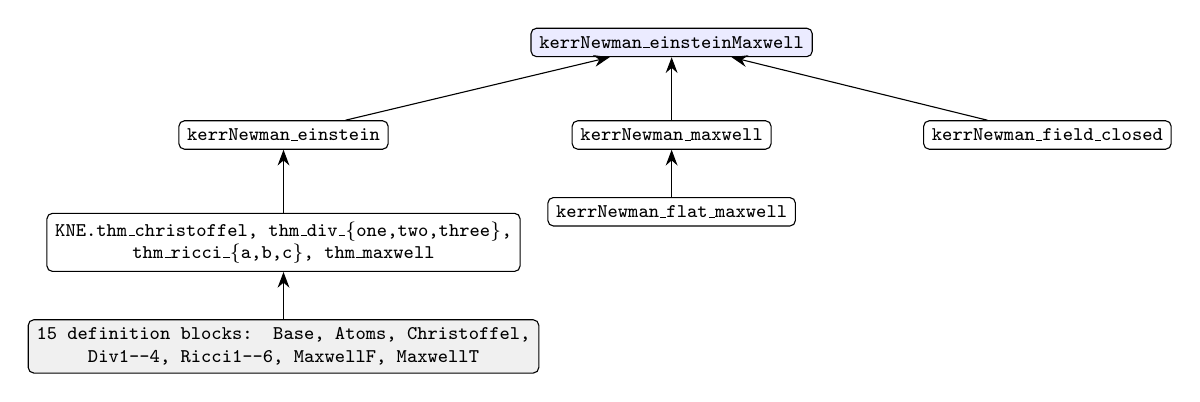
\begin{tikzpicture}[
  node distance=6mm and 4mm,
  box/.style={draw, rounded corners=2pt, font=\scriptsize\ttfamily, inner sep=3pt, align=center},
  blk/.style={box, fill=black!6},
  >={Stealth[length=2mm]}]
  \node[box, fill=blue!8] (em) {kerrNewman\_einsteinMaxwell};
  \node[box, below left=8mm and 18mm of em] (ein) {kerrNewman\_einstein};
  \node[box, below=8mm of em] (mx) {kerrNewman\_maxwell};
  \node[box, below right=8mm and 14mm of em] (fc) {kerrNewman\_field\_closed};
  \node[box, below=6mm of mx] (fm) {kerrNewman\_flat\_maxwell};
  \node[box, below=8mm of ein, align=center] (kne) {KNE.thm\_christoffel, thm\_div\_\{one,two,three\},\\ thm\_ricci\_\{a,b,c\}, thm\_maxwell};
  \node[blk, below=6mm of kne, align=center] (defs) {15 definition blocks: Base, Atoms, Christoffel,\\ Div1--4, Ricci1--6, MaxwellF, MaxwellT};
  \draw[->] (ein) -- (em);
  \draw[->] (mx) -- (em);
  \draw[->] (fc) -- (em);
  \draw[->] (fm) -- (mx);
  \draw[->] (kne) -- (ein);
  \draw[->] (defs) -- (kne);
\end{tikzpicture}
\caption{Dependency structure of the formal proof.
An arrow $A\to B$ means that the proof of $B$ uses~$A$.
Every node is a theorem or definition block checked on the platform.
The intermediate theorems \texttt{KNE.thm\_*} exist only so that each file checks within the time limit (\cref{sec:engineering}).}
\label{fig:deps}
\end{figure}

% ===========================================================================
\section{Kerr--Schild algebra in atoms}\label{sec:atoms}

\subsection{Atoms and relations}

Fix $p\in U$.
We call the following five real numbers the \emph{atoms} at~$p$:
\[
  r,\qquad k_1,\ k_2,\ k_3\quad(\text{the spatial components of }k),\qquad W:=\frac{1}{r^2+a^2k_3^2}.
\]
Since $k_3=z/r=\cos\theta$, we have $W=1/\Sigma$, the reciprocal of the Boyer--Lindquist function.

\begin{lemma}[\lean{ks_rel}, \lean{ks_W}, \lean{ks_x1}--\lean{ks_x3}, \lean{profile_eq}, \lean{pot_eq}]\label{lem:atoms}
At every point of $U$:
\begin{enumerate}[label=(\alph*)]
  \item $k_1^2+k_2^2+k_3^2=1$;
  \item $W\,(r^2+a^2k_3^2)=1$;
  \item $x=rk_1-ak_2$, $y=ak_1+rk_2$ and $z=rk_3$;
  \item $f=(2mr-e^2)\,W$ and $H:=er^3/(r^4+a^2z^2)=e\,r\,W$, so that $A=H\,k$.
\end{enumerate}
\end{lemma}
\begin{proof}[Proof sketch]
We have $(rx+ay)^2+(ry-ax)^2=(r^2+a^2)(x^2+y^2)$.
Hence $k_1^2+k_2^2=(x^2+y^2)/(r^2+a^2)$, and (a) is the first form of~\eqref{eq:quartic}.
Part (c) inverts the linear relations defining $k_1,k_2$.
Part (d) uses $r^4+a^2z^2=r^2(r^2+a^2k_3^2)$.
\end{proof}

\subsection{Derivatives of the atoms}

All atoms are independent of~$t$.
Implicit differentiation of~\eqref{eq:quartic} gives $\partial_x r = xr/(2r^2-\rho^2+a^2)$.
By~\eqref{eq:quartic}, $2r^2-\rho^2+a^2 = r^2+a^2k_3^2 = 1/W$.
Together with \cref{lem:atoms}(c) this yields
\begin{equation}\label{eq:dr}
  \partial_1 r = W r\,(rk_1-ak_2),\qquad
  \partial_2 r = W r\,(ak_1+rk_2),\qquad
  \partial_3 r = W k_3\,(r^2+a^2).
\end{equation}
The derivatives of $k_1,k_2,k_3$ and~$W$ are likewise polynomials in the atoms (\lean{dKt}, \lean{dWt}).
For instance, $\partial_1 k_1=Wr(k_2^2+k_3^2)$ and $\partial_3 k_3 = Wr(1-k_3^2)$.
For~$W$ we have $\partial_j W=-W^2\,(2r\,\partial_j r+2a^2k_3\,\partial_j k_3)$.

The algebraic content of these formulas is the following.
Let
\[
  \mathcal{P}=\Q[a,m,e][r,k_1,k_2,k_3,W],\qquad
  p_1=k_1^2+k_2^2+k_3^2-1,\qquad
  p_2=W(r^2+a^2k_3^2)-1,\qquad
  I=(p_1,p_2).
\]
Formulas~\eqref{eq:dr} and their analogues define derivations $D_1,D_2,D_3$ on~$\mathcal P$ that preserve~$I$.
This was checked symbolically; it is not needed in the formal proof.
So $\mathcal P/I$ is a differential ring, and evaluation at the atoms of a point $p\in U$ intertwines $D_j$ with~$\partial_j$.
The ring $\mathcal P/I$ is the localization of $\Q[a,m,e][r,k_1,k_2,k_3]/(p_1)$ at $\Sigma/r^2=r^2+a^2k_3^2$; the extra variable~$W$ is the Rabinowitsch device for inverting it.

\subsection{Kerr--Schild identities}

\begin{lemma}[\lean{ks_null}, \lean{det_KS}, \lean{mul_inv_KS}]\label{lem:ks}
Let $\ksharp:=\eta k=(-1,k_1,k_2,k_3)$ be the $\eta$-raised vector.
On~$U$ we have $\eta^{\mu\nu}k_\mu k_\nu=0$, $\det g=-1$ and
\[
  g^{-1}=\eta-f\,\ksharp\,\ksharp{}^{\!\top}.
\]
\end{lemma}
\begin{proof}
Nullity is \cref{lem:atoms}(a).
The determinant and the inverse are then checked by direct matrix computation; see~\cite{gurses1975,stephani2003} for the general Kerr--Schild statements.
\end{proof}

Hence every component of $g$, $g^{-1}$ and~$\partial g$ is (the evaluation of) an explicit element of~$\mathcal P$.
Since $\mathcal P$ is closed under the~$D_j$, so is every component of~$\Gamma$, $\partial\Gamma$, the Ricci tensor, $F$, $F^{\alpha\beta}$ and~$S_{\mu\nu}$.
No division is ever needed, because the only denominator, $r^2+a^2k_3^2$, has been absorbed into~$W$.
This is what makes the computation tractable in a proof assistant.

% ===========================================================================
\section{Certified polynomial identities}\label{sec:certificates}

\subsection{Ideal membership and Gr\"obner cofactors}

Every algebraic step of the proof has the following form.
Two explicit polynomials $L,R\in\mathcal P$ are given, for example the Christoffel formula applied to the closed forms of $g^{-1}$ and~$\partial g$ on one side, and a stored closed form on the other.
We must show $L=R$ at all real points satisfying $p_1=p_2=0$.
It suffices to find $c_1,c_2\in\mathcal P$ (or in its fraction field) with
\begin{equation}\label{eq:cert}
  L-R=c_1\,p_1+c_2\,p_2 .
\end{equation}

\begin{lemma}\label{lem:gb}
Order the variables lexicographically by $W>k_1>r>k_2>k_3>a>m>e$.
Then $\{p_1,p_2\}$ is a Gr\"obner basis of~$I$.
\end{lemma}
\begin{proof}
The leading monomials are $\LM(p_1)=k_1^2$ and $\LM(p_2)=Wr^2$, which are coprime.
By Buchberger's first criterion~\cite{buchberger1965,buchberger1979,cox2015}, the $S$-polynomial of $p_1$ and $p_2$ reduces to zero.
\end{proof}

Consequently, multivariate division of $L-R$ by $(p_1,p_2)$ returns quotients $c_1,c_2$ and a remainder.
The remainder is zero exactly when $L-R\in I$, and in that case the quotients satisfy~\eqref{eq:cert}.
We compute the division with SymPy's \texttt{reduced}~\cite{meurer2017}.
The generator stops with an error if the remainder is nonzero.

\subsection{Replay in Lean}

In Lean the relations are hypotheses
$\mathtt{hrel}:K_1^2+K_2^2+K_3^2=1$ and $\mathtt{hW}:W\,(R^2+a^2K_3^2)=1$ (Lean names \lean{R}, \lean{K1}, \ldots, \lean{W} for the atoms).
Each identity is closed by a single call such as
\begin{lstlisting}
theorem trGam_0 (a m e R K1 K2 K3 W : ℝ) (hrel : K1 ^ 2 + K2 ^ 2 + K3 ^ 2 = 1)
    (hW : W * (R ^ 2 + a ^ 2 * K3 ^ 2) = 1) :
    ∑ ρ, Gam a m e R K1 K2 K3 W ρ ρ 0 = 0 := by
  simp only [Gam, G000, G101, G202, G303, Matrix.cons_val, Fin.sum_univ_four]
  linear_combination (-2 * R^3 * W^3 * m^2 + 3 * R^2 * W^3 * m * e^2
      + 2 * R * K3^2 * W^3 * a^2 * m^2 - R * W^3 * e^4
      - K3^2 * W^3 * a^2 * m * e^2) * hrel + (0) * hW
\end{lstlisting}
(The exponent annotations \lean{(n : ℕ)} of the source have been dropped for readability.)
The tactic \lean{linear_combination}~\cite{mathlib_linear_combination} subtracts the given combination of the hypotheses from the goal.
It then closes the resulting equation with \lean{ring1}, Mathlib's normalizer for commutative rings~\cite{mathlib_ring,gregoire2005}, which produces a proof term checked by the kernel.
Nothing the computer algebra system computed is trusted.
A wrong cofactor makes \lean{ring1} fail and cannot produce a false theorem.
This is the ``skeptical'' combination of a proof assistant with an untrusted oracle~\cite{harrison1998}.
Mathlib's \lean{polyrith} tactic~\cite{mathlib_polyrith} applied the same idea one goal at a time: it sent the goal to SageMath through a web service and printed the resulting \lean{linear_combination} call. In the Mathlib version we use it is disabled because that service was shut down, which is one reason we compute the cofactors offline.
Our generators apply it offline and in bulk: the Einstein part contains \NumLCEinstein{} calls of \lean{linear_combination}.

\subsection{Why the extra atom \texorpdfstring{$W$}{W}}

An earlier version kept $1/(r^2+a^2k_3^2)$ as a denominator.
It closed identities with \lean{field_simp} followed by \lean{ring}.
On the larger expressions this was far too slow, because clearing denominators multiplies terms of high degree.
Making $W$ an independent variable linked to $r$ and $k_3$ by $p_2$ turns every rational identity into a polynomial one.
The cost is a second relation, which the Gr\"obner basis handles at no extra effort.
A few base lemmas still use \lean{field_simp} on small expressions, namely the derivative of the radius and the identities in \cref{lem:atoms}.

Each closed form stored in a definition block is chosen, among a few equivalent representatives modulo~$p_1$, to have the fewest monomials (\lean{best} in the generator).
It is written in a canonical expanded form.
The Base block holds 120 such definitions: 40 Christoffel symbols with up to 23 monomials each, 30 divergence terms $\partial_\rho\Gamma^\rho_{\nu\sigma}$ with up to 101 monomials, 10 Ricci components with up to 13 monomials, the field components and the invariant.
There are \NumCert{} certificates of the form $c_1\cdot\mathtt{hrel}+c_2\cdot\mathtt{hW}$ in the Einstein part.
Twenty-one of them, in the base lemmas, have rational cofactors and are normalized by \lean{field_simp}; 23 are trivial (both cofactors zero, so \lean{ring} alone would do); the remaining 118 have polynomial cofactors with a median of 32 monomials.
The largest certificate, for the $(1,2)$ component of the Ricci tensor, has 356 monomials, total degree 24, and occupies 28~kB of source.

% ===========================================================================
\section{Derivatives: a small calculus of coordinate partials}\label{sec:hascp}

The definitions use $\partial_k f(p)=Df(p)(e_k)$.
Rewriting with Mathlib's \lean{fderiv} lemmas on large expressions generates differentiability side goals.
It also manipulates continuous linear maps, which is slow.
We instead use a one-line predicate whose closure rules compute partial derivatives syntactically.

\begin{lstlisting}
/-- `f` is differentiable at `z` with coordinate partials `d k`. -/
structure HasCP (f : E4 → ℝ) (z : E4) (d : Fin 4 → ℝ) : Prop where
  diff : DifferentiableAt ℝ f z
  line : ∀ k, HasDerivAt (fun t : ℝ => f (z + t • coordBasis k)) (d k) 0

theorem HasCP.eq (h : HasCP f z df) (k : Fin 4) : coordPartial f k z = df k
\end{lstlisting}
\noindent The closure rules (\lean{HasCP.cst}, \lean{add}, \lean{sub}, \lean{neg}, \lean{mul}, \lean{div}, \lean{pow}) follow from the one-variable rules for \lean{HasDerivAt} along coordinate lines.
For example,
\[
  \texttt{HasCP.mul}:\ \ \mathsf{HasCP}\,f\,z\,d_f\ \wedge\ \mathsf{HasCP}\,g\,z\,d_g\ \Longrightarrow\ \mathsf{HasCP}\,(fg)\,z\,\big(k\mapsto d_f(k)\,g(z)+f(z)\,d_g(k)\big).
\]
A further rule, \lean{congr_d}, replaces the derivative by any pointwise-equal one.

\paragraph{Base cases.}
\lean{hasCP_R} differentiates the radius~\eqref{eq:r} along coordinate lines.
It needs $r>0$ and positivity of the inner square root, and it is matched to~\eqref{eq:dr} by a certificate.
\lean{hasCP_K1}--\lean{hasCP_K3}, \lean{hasCP_W}, \lean{hasCP_profile} and \lean{hasCP_H} follow, all with derivatives in atom form.

\paragraph{Generated derivations.}
Each Christoffel closed form is a polynomial $P$ in the atoms.
To obtain $\partial_\rho$ of $p\mapsto P(\text{atoms}(p))$, the generator emits a \lean{HasCP} proof term built from the closure rules.
The term follows the same syntax tree that was used to print~$P$: a balanced binary sum of monomials.
Lean therefore accepts the term by unfolding definitions, with no rewriting.
The derivative it produces is the chain-rule expansion, which \lean{congr_d} together with one certificate identifies with the stored closed form of the divergence term.
The Lean statement is \lean{dG112}, for instance, which gives both differentiability and the value of $\partial_1$ of the component $\Gamma^1_{12}$.
The thirty-four generated derivations contain 5{,}286 applications of the closure rules in total; the largest single term is about 4~kB.

\begin{lemma}[\lean{cp_time}]\label{lem:time}
For any $\Phi:\R^4\to\R$, the function $p\mapsto\Phi(r(p),k_1(p),k_2(p),k_3(p))$ has $\partial_0=0$ everywhere.
\end{lemma}
\begin{proof}
The function is invariant under $p\mapsto p+t e_0$.
If it is differentiable at~$p$, its derivative along~$e_0$ is that of a constant.
If not, the Fr\'echet derivative is~$0$ by convention.
\end{proof}

\paragraph{From local identities to derivatives.}
The proof shows that the platform's Christoffel symbols equal the closed form \lean{Gam} evaluated at the atoms, at every point of $U$ (\lean{thm_christoffel}).
Because $U$ is open, the two functions agree near any $p\in U$, so their derivatives at~$p$ agree (\lean{Filter.EventuallyEq.fderiv_eq}).
This is how derivatives of the platform's \lean{christoffel} reduce to derivatives of closed forms.

% ===========================================================================
\section{The Einstein equation}\label{sec:einstein}

Fix $p\in U$ and write $\Gamma$, $D^\rho_{\nu\sigma}:=\partial_\rho\Gamma^\rho_{\nu\sigma}$ (no sum) and so on for the closed forms evaluated at the atoms of~$p$.

\paragraph{Christoffel symbols.}
By \cref{lem:ks}, $g^{-1}$ is polynomial in the atoms.
With the \lean{HasCP} derivatives of $g=\eta+f\,k\otimes k$ (\lean{cp_metric}), the Christoffel formula becomes a polynomial expression.
Forty certificates, one for each $\Gamma^i_{jk}$ with $j\le k$, identify it with the stored closed forms (\lean{thm_christoffel}).

\paragraph{Ricci tensor.}
Unfolding the definitions,
\begin{equation}\label{eq:ricci}
  R_{\sigma\nu}=\sum_\rho\partial_\rho\Gamma^\rho_{\nu\sigma}
  -\partial_\nu\Big(\sum_\rho\Gamma^\rho_{\rho\sigma}\Big)
  +\sum_{\rho,\lambda}\Gamma^\rho_{\rho\lambda}\Gamma^\lambda_{\nu\sigma}
  -\sum_{\rho,\lambda}\Gamma^\rho_{\nu\lambda}\Gamma^\lambda_{\rho\sigma}.
\end{equation}
The contracted symbol $\sum_\rho\Gamma^\rho_{\rho\sigma}=\frac12\partial_\sigma\log|\det g|$ vanishes on~$U$ because $\det g=-1$.
In the formal proof this is not derived from the determinant.
It is checked directly on the closed forms by four certificates (\lean{trGam}).
Since the trace vanishes on the open set~$U$ and each summand is differentiable (\lean{diff_tr}), the second term of~\eqref{eq:ricci} is zero, and so is the third.
The first term is given by the divergence closed forms.
For $\rho=0$ it vanishes by \cref{lem:time}.
For $\rho=1,2,3$ it comes from the thirty generated derivations (\lean{thm_div_one}--\lean{thm_div_three}).
The remaining expression is identified with a closed-form Ricci tensor \lean{RicA} by ten certificates, one for each component with $\sigma\le\nu$ (\lean{thm_ricci_a}--\lean{thm_ricci_c}).
The other six components follow by symmetry.

\paragraph{Scalar curvature.}
One certificate shows $\sum_{\sigma,\nu}g^{\sigma\nu}R_{\sigma\nu}=0$ (\lean{scal_zero}).
This reflects the tracelessness of the Maxwell stress tensor in four dimensions.
Hence $G_{\mu\nu}=R_{\mu\nu}$ at~$p$.

\paragraph{The source.}
Using the \lean{HasCP} rules for $A=Hk$, the field $F_{\mu\nu}=\partial_\mu(Hk_\nu)-\partial_\nu(Hk_\mu)$ is put in closed form (\lean{field_closed} in the final file).
Further certificates give $F^{\alpha\beta}$, the invariant $F_{\alpha\beta}F^{\alpha\beta}$ and finally $S_{\mu\nu}$ in closed form.
The last step identifies $S_{\mu\nu}$ with the same polynomial \lean{RicA} (\lean{thm_maxwell}).

\paragraph{Conclusion.}
The final file chains these facts:
\begin{lstlisting}
theorem einstein_eq (m a e : ℝ) (y : E4) (hy : 0 < ksRadius a y) (μ ν : Fin 4) :
    einsteinTensor (kerrNewmanMetric m a e) y μ ν
      = RicA a m e (ksRadius a y) (ksNull a y 1) (ksNull a y 2) (ksNull a y 3) (Wf a y) μ ν
theorem maxwell_eq (m a e : ℝ) (y : E4) (hy : 0 < ksRadius a y) (μ ν : Fin 4) :
    maxwellSource (kerrNewmanMetric m a e) (kerrNewmanField a e) y μ ν
      = RicA a m e (ksRadius a y) (ksNull a y 1) (ksNull a y 2) (ksNull a y 3) (Wf a y) μ ν
\end{lstlisting}
\noindent The Einstein equation~(i) is then a single rewrite.
Before any Lean code was generated, the same symbolic pipeline verified $G_{\mu\nu}=S_{\mu\nu}$ and $R=0$ in SymPy, and spot checks were made at random numerical points.
These checks guided development but play no role in the formal proof.

% ===========================================================================
\section{The Maxwell equations}\label{sec:maxwell}

\subsection{Closedness}

For any potential $A$ that is $C^2$ near~$p$, the three terms of $\partial_{[\lambda}F_{\mu\nu]}$ cancel pairwise by symmetry of second derivatives.
Mathlib provides this symmetry as \lean{ContDiffAt.isSymmSndFDerivAt}.
Smoothness of $A$ on~$U$ is discharged by Mathlib's \lean{fun_prop}, given that $r>0$, that $r^2+a^2\neq0$ and $r^4+a^2z^2\neq0$, and that the discriminant in~\eqref{eq:r} is positive.
The whole proof (\lean{kerrNewman_field_closed}) is \NumLinesFieldClosed{} lines.

\subsection{From curved to flat space}\label{sec:curved-to-flat}

\begin{proposition}[\lean{star_eq}]\label{prop:flat}
On~$U$, $\sqrt{|\det g|}\,F^{\mu\nu}=\eta^{\mu\alpha}\eta^{\nu\beta}F_{\alpha\beta}$.
\end{proposition}
\begin{proof}
By \cref{lem:ks}, $\sqrt{|\det g|}=1$ and $g^{-1}=P:=\eta-f\,\ksharp\ksharp{}^{\!\top}$.
Write $F=d(Hk)$.
\begin{enumerate}[label=(\roman*)]
  \item Contracting $F_{\mu\nu}=\partial_\mu H\,k_\nu-\partial_\nu H\,k_\mu+H(\partial_\mu k_\nu-\partial_\nu k_\mu)$ with $\ksharp{}^\nu$ uses three facts.
  First, $k_\nu\ksharp{}^\nu=0$ (nullity).
  Second, $\ksharp{}^\nu\partial_\mu k_\nu=\frac12\partial_\mu(\eta^{\alpha\beta}k_\alpha k_\beta)=0$.
  Third, $\ksharp{}^\nu\partial_\nu k_\mu=0$, i.e.\ $\ksharp$ is geodesic for~$\eta$; this is checked with~\eqref{eq:dr}.
  Together they give the alignment
  \[
    F_{\mu\nu}\,\ksharp{}^\nu=\lambda\,k_\mu,\qquad \lambda=-\ksharp{}^\nu\partial_\nu H .
  \]
  \item By antisymmetry, $\ksharp{}^{\!\top}F=-\lambda\,k^{\top}$.
  Using $\eta k=\ksharp$, we get $\eta F\ksharp=\lambda\ksharp$, $\ksharp{}^{\!\top}F\eta=-\lambda\ksharp{}^{\!\top}$ and $\ksharp{}^{\!\top}F\ksharp=0$.
  Hence
  \begin{align*}
    PFP^{\top}&=\eta F\eta-f\,\ksharp(\ksharp{}^{\!\top}F\eta)-f\,(\eta F\ksharp)\ksharp{}^{\!\top}+f^2\,\ksharp(\ksharp{}^{\!\top}F\ksharp)\ksharp{}^{\!\top}\\
    &=\eta F\eta+f\lambda\,\ksharp\ksharp{}^{\!\top}-f\lambda\,\ksharp\ksharp{}^{\!\top}=\eta F\eta.\qedhere
  \end{align*}
\end{enumerate}
\end{proof}
\noindent Since the identity holds on the open set~$U$, the divergences of both sides agree at every $p\in U$.
The curved Maxwell equation~(ii) is thus equivalent to the flat one, $\partial_\mu(\eta^{\mu\alpha}\eta^{\nu\beta}F_{\alpha\beta})=0$.
This proof (\lean{kerrNewman_maxwell}, \NumLinesMaxwell{} lines) does not use the atom machinery.
\Cref{prop:flat} is closely related to the Kerr--Schild double copy~\cite{monteiro2014}, in which the gauge field $\phi k$ built from a stationary Kerr--Schild metric solves the flat Maxwell equations.

\subsection{The flat Maxwell equation}\label{sec:flat}

All fields are $t$-independent.
Write $A=(H,\vec A)$ with $\vec A=H\,\vec k$.
The $\nu=0$ component of the flat equation is $-\Delta H=0$.
The $\nu=i$ components are $\sum_j\partial_j(\partial_jA_i-\partial_iA_j)=-(\nabla\times\nabla\times\vec A)_i=0$.
We prove two identities on~$U$:
\begin{equation}\label{eq:flat}
  \Delta H=0,\qquad \nabla\times\vec A=\nabla\psi,\qquad \psi:=\frac{e\,a\,z\,r}{r^4+a^2z^2}.
\end{equation}
The second implies $\nabla\times\nabla\times\vec A=\nabla\times\nabla\psi=0$, by symmetry of the second derivatives of the smooth function~$\psi$.
Both identities in~\eqref{eq:flat} are verified componentwise in Lean.
Each component is an explicit derivative computation (along coordinate lines, as in \cref{sec:hascp}) followed by \lean{field_simp}, \lean{ring} and \lean{linear_combination} with the quartic relation~\eqref{eq:quartic}.
The proof (\lean{kerrNewman_flat_maxwell}) is \NumLinesFlatMaxwell{} lines.

\paragraph{Interpretation.}
The pair $(H,\psi)$ is the real and imaginary part of Appell's potential~\cite{appell1887}, the Coulomb potential of a charge placed at the imaginary point $(0,0,ia)$:
\[
  H+i\psi=\frac{e\,r}{r^2-iaz}=\frac{e}{r-iaz/r}=\frac{e}{\sqrt{x^2+y^2+(z-ia)^2}} .
\]
The last equality uses $(r-iaz/r)^2=x^2+y^2+(z-ia)^2$, which follows from~\eqref{eq:quartic}, and picks the root with positive real part~$r$.
This is the classical picture of the Kerr--Newman field as the field of a complex-shifted point charge~\cite{newman1973,lyndenbell2003,adamo2014}.
In this picture $\Delta H=0$ is the harmonicity of the real part of a harmonic function.
The formal proof does not use complex numbers; it verifies~\eqref{eq:flat} directly.

% ===========================================================================
\section{Engineering a large proof under a time budget}\label{sec:engineering}

\subsection{Platform constraints}

Prove2Me checks each submission on its server within 300 seconds.
This budget includes building any platform modules the submission imports that are not already cached.
Submissions may not define new syntax or tactics (no \lean{macro} or \lean{syntax} commands).
The platform distinguishes \emph{definition blocks}, which are published modules that other files may import and which may contain lemmas, from \emph{theorems}.
A proof may import a theorem's statement and use it as an axiom-free reduction that the platform tracks.
That theorem's own proof is checked separately.

Our first complete proof of the Einstein equation was a single file of about 2{,}650 lines.
It needed more than 13~GB of memory and more than 300~seconds on our machine, and the platform ran out of memory while rebuilding its dependencies.
The final development (\cref{tab:blocks}) splits the work along the natural stages of the computation.
\begin{itemize}
  \item Fifteen definition blocks hold the closed forms, the \lean{HasCP} base lemmas and the heavy certified lemmas.
  \item Eight intermediate theorems restate the needed facts over the closed forms.
  Their proofs are a few lines that \lean{exact} lemmas from the blocks.
  \item A final file of \NumLinesFinal{} lines imports only the two light blocks and the eight theorem statements, and assembles the result.
\end{itemize}
The heaviest block now checks in 76~seconds, and the whole Einstein part in about ten minutes of elaboration time. Generating the Lean source takes about four and a half minutes of SymPy time, the bulk of it in the symbolic curvature computation that doubles as an independent check. The generated fragments are 94\% of the Einstein part by volume; the rest is hand-written glue.

\begin{table}[t]
\centering
\footnotesize
\setlength{\tabcolsep}{3.5pt}
\begin{tabular}{@{}llrrrrr@{}}
\toprule
File & Content & Lines & kB & Lemmas & Certif. & Check (s) \\
\midrule
\multicolumn{7}{@{}l}{\emph{Definition blocks}}\\
Base & atoms, \lean{HasCP} calculus, 120 closed forms & 798 & 245 & 51 & -- & 28 \\
Atoms & \lean{HasCP} for $r,k_i,W,f,H$; $g$, $g^{-1}$, $\Gamma$ & 256 & 20 & 12 & 28 & 26 \\
Christoffel & 40 identities $\Gamma^i_{jk}=$ closed form & 310 & 96 & 46 & 40 & 74 \\
Div1 & $\partial_0$ differentiability; $\partial_1\Gamma^1_{0\sigma}$ & 142 & 36 & 8 & 4 & 20 \\
Div2 & $\partial_1\Gamma^1_{\nu\sigma}$, $1\le\nu\le\sigma$ & 150 & 82 & 6 & 6 & 73 \\
Div3 & $\partial_2\Gamma^2_{\nu\sigma}$ & 238 & 85 & 10 & 10 & 76 \\
Div4 & $\partial_3\Gamma^3_{\nu\sigma}$ & 238 & 63 & 10 & 10 & 49 \\
Ricci1--6 & 10 identities $R_{\sigma\nu}=$ closed form & 168 & 232 & 10 & 10 & 205 \\
MaxwellF & $F$, $F^{\alpha\beta}$, $F_{\alpha\beta}F^{\alpha\beta}$ in closed form & 223 & 19 & 35 & 33 & 18 \\
MaxwellT & 16 identities $S_{\mu\nu}=$ closed form & 118 & 70 & 17 & 16 & 41 \\
\midrule
\multicolumn{7}{@{}l}{\emph{Theorems}}\\
\texttt{KNE.thm\_*} (8) & restatements over the blocks & 193 & 10 & 8 & -- & $<1$ \\
\texttt{kerrNewman\_einstein} & assembly (\cref{sec:einstein}) & 251 & 17 & 28 & 5 & 3 \\
\texttt{kerrNewman\_field\_closed} & $dF=0$ & 88 & 4 & 7 & -- & 1 \\
\texttt{kerrNewman\_flat\_maxwell} & flat Maxwell (\cref{sec:flat}) & 720 & 35 & 79 & -- & 8 \\
\texttt{kerrNewman\_maxwell} & reduction to flat (\cref{sec:curved-to-flat}) & 460 & 23 & 48 & -- & 16 \\
\texttt{kerrNewman\_einsteinMaxwell} & milestone & 15 & 1 & 1 & -- & $<1$ \\
\midrule
Total & & \TotalLines & \TotalKB & 376 & \NumCert & 639 \\
\bottomrule
\end{tabular}
\caption{The files of the formal proof.
``Lemmas'' counts top-level theorems and lemmas; ``Certif.'' counts \lean{linear_combination} certificates of the form $c_1\cdot\mathtt{hrel}+c_2\cdot\mathtt{hW}$ (the Ricci and Maxwell rows also contain a few hand-written ones).
``Check'' is the wall-clock time to re-elaborate the file against compiled imports, net of the 7.6~s needed to load Mathlib, minimum of two runs on a 4-core 2.1~GHz machine with 15~GB of memory.
Peak memory was 6.4--8.4~GB per file, almost all of it the memory-mapped Mathlib library.}
\label{tab:blocks}
\end{table}

\subsection{Lessons}

Several low-level choices mattered as much as the overall design.
\begin{itemize}
  \item \emph{Annotate exponents.}
  Writing \lean{R ^ (4 : ℕ)} instead of \lean{R ^ 4} in generated polynomials avoided slow elaboration of the many \lean{^} occurrences under Lean's default-instance mechanism.
  \item \emph{One definition per closed form.}
  A single table holding all forty Christoffel symbols exceeded the heartbeat limit during elaboration; one \lean{def} per entry did not.
  \item \emph{Print and prove from the same tree.}
  The \lean{HasCP} terms are generated from the expression tree used to print the definition they differentiate.
  The two then agree by definitional unfolding, and no rewriting is needed.
  Mismatched association of sums was the main source of early type errors.
  \item \emph{Exploit symmetry.}
  Only components with $j\le k$ of $\Gamma^i_{jk}$ and $\sigma\le\nu$ of $R_{\sigma\nu}$ are certified.
  The symmetry lemmas themselves are proved by \lean{rfl} or by unfolding \lean{Matrix.cons_val} with \lean{simp only}.
  \item \emph{Prefer polynomial identities.}
  As explained in \cref{sec:certificates}, replacing \lean{field_simp} by polynomial certificates was decisive for speed.
\end{itemize}

% ===========================================================================
\section{Trusted base and validation}\label{sec:trust}

\paragraph{What is checked.}
For the final theorem and for the milestone, \lean{#print axioms} reports
\begin{lstlisting}[basicstyle=\ttfamily\footnotesize]
'NoHair.kerrNewman_einsteinMaxwell' depends on axioms: [propext, Classical.choice, Quot.sound]
\end{lstlisting}
No \lean{sorry}, \lean{admit}, \lean{native_decide} or \lean{axiom} occurs anywhere in the \TotalLines{} lines of proof, and no heartbeat limit is raised.
Every file was checked by the Prove2Me server with the platform's toolchain.
On the platform each theorem is checked against \lean{sorry}-stubs of the theorems it imports, so the platform's verdict is compositional. We also rebuilt the whole chain locally in a single Lean environment, with every stub replaced by its accepted proof under the platform name, and ran \lean{#print axioms} on the milestone and on each of its three conjuncts; all four report exactly the three axioms above. The scripts for this check are in the repository.

\paragraph{What must be trusted.}
To believe \cref{thm:main} one must trust the Lean kernel and the Mathlib definitions involved: \lean{fderiv}, matrix inverse and determinant, \lean{Real.sqrt}.
One must also accept that the platform definitions of \cref{sec:defs,sec:kn} express the intended notions.
These are about 150 lines, reproduced in \cref{app:defs}.
We compared them with the standard references (\cref{sec:defs}).
The generators, SymPy and the AI agent that wrote the proofs need not be trusted.
Neither does the reader need to inspect the roughly one megabyte of generated proof text.

\paragraph{Limitations.}
The statement is coordinate-based and pointwise.
It does not use Mathlib's manifold library, which does not yet provide pseudo-Riemannian curvature.
It covers the $r>0$ sheet of the Kerr--Schild chart.
It concerns only the \emph{existence} side of the no-hair story, namely that Kerr--Newman is a solution.
The uniqueness theorems, which are the mission's real goal, are far beyond the present work.
Another milestone, \lean{NoHair.kerrNewman_isStationaryBlackHole}, which asserts that the Kerr--Newman spacetime satisfies the global hypotheses of the uniqueness theorem, is not addressed here.
Finally, the generated proof is optimized for checkability, not readability.
The human-readable content is the method described above together with the generators.

% ===========================================================================
\section{Related work}\label{sec:related}

\paragraph{Computer algebra in general relativity.}
Verifying exact solutions is a classical application of computer algebra; see MacCallum's review~\cite{maccallum2018}.
It is supported by dedicated systems such as xAct~\cite{martingarcia2008}, Cadabra~\cite{peeters2007} and SageManifolds~\cite{gourgoulhon2015}, as well as general-purpose systems.
The catalogue of Stephani et al.~\cite{stephani2003} relies on such checks.
These tools produce results, not proofs.
Our pipeline uses SymPy in exactly this role, but only to find certificates that Lean then checks.

\paragraph{Certificates from untrusted oracles.}
Combining a proof assistant with an external algebra system that supplies checkable witnesses goes back at least to Harrison and Th\'ery~\cite{harrison1998}.
Later instances include the use of Maple from Coq~\cite{delahaye2005} and certified computer algebra on top of a prover~\cite{kaliszyk2007}.
Mathlib's \lean{polyrith}~\cite{mathlib_polyrith} found \lean{linear_combination} coefficients with an external system. Gr\"obner-basis certificates have been used for ring identities in Isabelle~\cite{chaieb2007} and HOL~Light~\cite{harrison2007}, and Buchberger's algorithm itself has been verified in Coq~\cite{thery2001}. Coq's \texttt{nsatz} checks certificates produced by external Gr\"obner computations~\cite{pottier2010}. Lean has been connected to Mathematica~\cite{lewis2022}, and recent work develops Gr\"obner-based tactics and Gr\"obner theory in Lean~4~\cite{shen2026tactics,guo2026groebner}.
Our use of Gr\"obner-basis cofactors as certificates is standard.
What is specific here is the reduction of an entire curvature computation to ideal membership in a small differential ring of atoms.

\paragraph{Formalized physics and relativity.}
Formal treatments of relativity have so far been mostly axiomatic or kinematic. Stannett and N\'emeti verified results of first-order axiomatic relativity in Isabelle/HOL~\cite{stannett2014}, and Schutz's axioms for Minkowski spacetime have been formalized there as well~\cite{schmoetten2021}. In Lean~4, the HepLean project (now Physlib)~\cite{toobysmith2025heplean,toobysmith2024index,physlib} formalizes parts of high-energy physics, tensor index notation and special relativity. Recent work proves analytic results on a fixed black-hole background~\cite{kehle2026rn}, taking the metric as given. We are not aware of an earlier formal proof that the Schwarzschild, Kerr or Kerr--Newman metric satisfies the Einstein equations with the curvature computed from the metric through the prover's own analysis library. Our searches of the literature and of public code repositories (October 2026) found none.

% ===========================================================================
\section{Conclusion}\label{sec:conclusion}

We have given a complete machine-checked proof that the Kerr--Newman metric and field solve the Einstein--Maxwell equations.
The definitions are elementary and the region is the full $r>0$ part of the Kerr--Schild chart.
The approach combines a choice of atoms that makes the solution's algebra polynomial and closed under differentiation, cheap certificates from an untrusted Gr\"obner-basis computation, and a small differentiation calculus.
It should transfer to other exact solutions whose metric components lie in a finitely generated differential algebra with a few relations.
Natural next targets are Kerr--Schild metrics more generally and accelerating or NUT-charged solutions.
On the conceptual side, connecting the coordinate statement to a manifold-level Lorentzian geometry library would make the result reusable in the mission's harder milestones.

\section*{Acknowledgements and use of AI tools}
The Lean proofs, the SymPy generators and a first draft of this manuscript were produced by Claude Code, an AI coding agent developed by Anthropic.
The agent worked under the author's direction on the Prove2Me platform.
The formal statement and definitions were authored by the Prove2Me mission authors.
All formal claims were checked by the Lean kernel.
The author takes responsibility for the content of this paper.

\section*{Data availability}
The complete development is publicly available in the repository
\begin{center}\url{https://github.com/SamenSHossain/math-solver}\end{center}
in the directory \texttt{prove2me/nohair/}, which holds all Lean files, the Python generators and the definition blocks.
The platform objects are listed in \cref{app:ids} and can be inspected on \url{https://prove2.me}.
The directory \texttt{paper/kerr-newman/} contains the source of this paper, the scripts that reproduce the statistics and the single-environment axiom check, and the audit scripts for the conventions of \cref{sec:defs}. The Lean toolchain was version 4.33.1 with Mathlib commit \texttt{0df444a3}.

\bibliographystyle{plainnat}
\bibliography{refs}

% ===========================================================================
\appendix
\section{The platform definitions}\label{app:defs}

These definitions are reproduced verbatim from the Prove2Me definition blocks \texttt{NoHair\_coordinates} and \texttt{NoHair\_kerrNewman}; docstrings are shortened.
They are everything \cref{thm:main} depends on beyond Mathlib.

\begin{lstlisting}
abbrev E4 := EuclideanSpace ℝ (Fin 4)
def coordBasis (μ : Fin 4) : E4 := EuclideanSpace.single μ 1
def minkowski : Matrix (Fin 4) (Fin 4) ℝ := Matrix.diagonal ![-1, 1, 1, 1]
def coordPartial (f : E4 → ℝ) (k : Fin 4) (y : E4) : ℝ := fderiv ℝ f y (coordBasis k)
def invMetric (G : E4 → Matrix (Fin 4) (Fin 4) ℝ) (y : E4) : Matrix (Fin 4) (Fin 4) ℝ :=
  (G y)⁻¹

def christoffel (G : E4 → Matrix (Fin 4) (Fin 4) ℝ) (y : E4) (i j k : Fin 4) : ℝ :=
  ∑ l, (1 / 2 : ℝ) * invMetric G y i l *
    (coordPartial (fun z => G z l k) j y + coordPartial (fun z => G z l j) k y
      - coordPartial (fun z => G z j k) l y)

def riemann (G : E4 → Matrix (Fin 4) (Fin 4) ℝ) (y : E4) (ρ σ μ ν : Fin 4) : ℝ :=
  coordPartial (fun z => christoffel G z ρ ν σ) μ y
    - coordPartial (fun z => christoffel G z ρ μ σ) ν y
    + ∑ l, (christoffel G y ρ μ l * christoffel G y l ν σ
      - christoffel G y ρ ν l * christoffel G y l μ σ)

def ricci (G : E4 → Matrix (Fin 4) (Fin 4) ℝ) (y : E4) (σ ν : Fin 4) : ℝ :=
  ∑ ρ, riemann G y ρ σ ρ ν

def scalarCurvature (G : E4 → Matrix (Fin 4) (Fin 4) ℝ) (y : E4) : ℝ :=
  ∑ σ, ∑ ν, invMetric G y σ ν * ricci G y σ ν

def einsteinTensor (G : E4 → Matrix (Fin 4) (Fin 4) ℝ) (y : E4) (μ ν : Fin 4) : ℝ :=
  ricci G y μ ν - (1 / 2 : ℝ) * scalarCurvature G y * G y μ ν

def raiseBoth (G : E4 → Matrix (Fin 4) (Fin 4) ℝ) (F : E4 → Matrix (Fin 4) (Fin 4) ℝ)
    (y : E4) (α β : Fin 4) : ℝ :=
  ∑ μ, ∑ ν, invMetric G y α μ * invMetric G y β ν * F y μ ν

def maxwellSource (G : E4 → Matrix (Fin 4) (Fin 4) ℝ) (F : E4 → Matrix (Fin 4) (Fin 4) ℝ)
    (y : E4) (μ ν : Fin 4) : ℝ :=
  2 * ((∑ α, ∑ β, F y μ α * invMetric G y α β * F y ν β)
    - (1 / 4 : ℝ) * G y μ ν * ∑ α, ∑ β, F y α β * raiseBoth G F y α β)

def EinsteinMaxwellAt (G : E4 → Matrix (Fin 4) (Fin 4) ℝ) (F : E4 → Matrix (Fin 4) (Fin 4) ℝ)
    (y : E4) : Prop :=
  (∀ μ ν, einsteinTensor G y μ ν = maxwellSource G F y μ ν) ∧
  (∀ ν, ∑ μ, coordPartial
      (fun z => Real.sqrt |(G z).det| * raiseBoth G F z μ ν) μ y = 0) ∧
  (∀ l μ ν, coordPartial (fun z => F z μ ν) l y + coordPartial (fun z => F z ν l) μ y
      + coordPartial (fun z => F z l μ) ν y = 0)

def ksRadius (a : ℝ) (y : E4) : ℝ :=
  let ρ2 := y 1 ^ 2 + y 2 ^ 2 + y 3 ^ 2
  Real.sqrt ((ρ2 - a ^ 2 + Real.sqrt ((ρ2 - a ^ 2) ^ 2 + 4 * a ^ 2 * y 3 ^ 2)) / 2)

def ksNull (a : ℝ) (y : E4) : Fin 4 → ℝ :=
  let r := ksRadius a y
  ![1, (r * y 1 + a * y 2) / (r ^ 2 + a ^ 2), (r * y 2 - a * y 1) / (r ^ 2 + a ^ 2), y 3 / r]

def ksProfile (m a e : ℝ) (y : E4) : ℝ :=
  let r := ksRadius a y
  r ^ 2 * (2 * m * r - e ^ 2) / (r ^ 4 + a ^ 2 * y 3 ^ 2)

def kerrNewmanMetric (m a e : ℝ) (y : E4) : Matrix (Fin 4) (Fin 4) ℝ :=
  fun μ ν => minkowski μ ν + ksProfile m a e y * ksNull a y μ * ksNull a y ν

def kerrNewmanPotential (a e : ℝ) (y : E4) : Fin 4 → ℝ :=
  let r := ksRadius a y
  fun μ => e * r ^ 3 / (r ^ 4 + a ^ 2 * y 3 ^ 2) * ksNull a y μ

def kerrNewmanField (a e : ℝ) (y : E4) : Matrix (Fin 4) (Fin 4) ℝ :=
  fun μ ν => coordPartial (fun z => kerrNewmanPotential a e z ν) μ y
    - coordPartial (fun z => kerrNewmanPotential a e z μ) ν y
\end{lstlisting}

\section{Platform objects}\label{app:ids}

\begin{center}
\small
\begin{tabular}{@{}ll@{}}
\toprule
Platform theorem (all status \emph{Proved}) & Identifier \\
\midrule
\texttt{NoHair.kerrNewman\_einsteinMaxwell} & \texttt{35932774-6f3d-4986-915d-e2e8baec247a} \\
\texttt{NoHair.kerrNewman\_einstein} & \texttt{29511860-2b59-4995-a0aa-33f3e4ef6f27} \\
\texttt{NoHair.kerrNewman\_maxwell} & \texttt{c5c86a9f-be51-4ff0-b03c-7af1195b1b3b} \\
\texttt{NoHair.kerrNewman\_flat\_maxwell} & \texttt{2a76a228-69dd-4f40-a775-d8e98e4f6349} \\
\texttt{NoHair.kerrNewman\_field\_closed} & \texttt{9c810d9f-30fa-4607-8131-cb6b04375499} \\
\texttt{NoHair.KNE.thm\_christoffel} & \texttt{8dcd053d-2b42-4da1-b938-e3b583380372} \\
\texttt{NoHair.KNE.thm\_div\_one} & \texttt{6c168c47-f9a1-4c51-8479-700ca0814cee} \\
\texttt{NoHair.KNE.thm\_div\_two} & \texttt{36d617c4-dee0-4ad2-a404-b36e7ef9f8df} \\
\texttt{NoHair.KNE.thm\_div\_three} & \texttt{05c945f9-3d3d-4c04-b90f-a76537cfef0c} \\
\texttt{NoHair.KNE.thm\_ricci\_a} & \texttt{97f00edb-2452-4ddf-bc82-400a0b9946d5} \\
\texttt{NoHair.KNE.thm\_ricci\_b} & \texttt{eb386bc8-000f-4b46-b331-5014c2f82f08} \\
\texttt{NoHair.KNE.thm\_ricci\_c} & \texttt{e9f7c9ec-a103-4680-885e-9110e2332bfc} \\
\texttt{NoHair.KNE.thm\_maxwell} & \texttt{a193ccd8-906e-420e-9057-670b9556dc7e} \\
\bottomrule
\end{tabular}
\end{center}
The fifteen definition blocks are published as \texttt{NoHair\_KerrNewmanEinstein\_}$X$ for $X$ one of Base, Atoms, Christoffel, Div1--Div4, Ricci1--Ricci6, MaxwellF and MaxwellT.

\end{document}
